% ==============================================================================
% LAB 118
% GRUNDLÄGGNADE MÄTINSTUMENT
% --------------------------
% Last updated <2015-02-18> 
%
% Author:
% Jonas Sjöberg     <tel12jsg@student.hig.se>
% Oscar Wallberg    <tco13owg@student.hig.se>
% 
% License:
% Creative Commons Attribution-NonCommercial-ShareAlike 4.0 International
% See LICENSE.md for full licensing information.
% ==============================================================================

% ==============================================================================
% INCLUDES AND CONFIGURATION
% ==============================================================================
\documentclass[11pt,a4paper]{article}
\usepackage[utf8]{inputenc}
\usepackage[swedish]{babel} % För svensk innehållsförteckning
\usepackage{siunitx} % (För dokumentation, kör i terminalen; texdoc siunitx)
\usepackage{amssymb}
\usepackage{amsmath}
\usepackage{amsfonts}
\usepackage{graphicx}
\usepackage{booktabs}
\usepackage{longtable} % Tables span across pages
\usepackage{microtype}
\usepackage{gensymb}
%\usepackage{tabto}
\usepackage{units}

\setlength\parindent{0pt} % Removes all indentation from paragraphs

% ==============================================================================
% DOCUMENT METADATA 
% ==============================================================================
\title{EE466 \\ Lab 118 \\ Grundläggande Mätinstrument}

\author{\\
  Jonas Sjöberg\\
  Högskolan i Gävle,\\
  Elektronikingenjörsprogrammet,\\
  \texttt{tel12jsg@student.hig.se}\\
  \\
  Oscar Wallberg\\
  Högskolan i Gävle,\\
  Dataingenjörsprogrammet,\\
  \texttt{tco13owg@student.hig.se}\\}

\date{}
% ==============================================================================
\begin{document}
% ==============================================================================
\maketitle

\begin{center}
    \begin{tabular}{l r}
        Labb utförd: & 6 Februari 2015 \\
        Instruktör: & Efrain Zenteno
    \end{tabular}
\end{center}

% ==============================================================================
% ABSTRACT
% ==============================================================================
\begin{abstract}
    Syftet med laborationen är att lära känna de vanligaste basinstrumenten i
    ett elektroniklaboratorium och innefattar övningar i att hantera
    oscilloskop, multimeter, nätaggregat, och funktionsgenerator.
\end{abstract}

\newpage

{
    %\hypersetup{linkcolor=black}
    \setcounter{tocdepth}{3}
    \tableofcontents
}

\newpage

% ==============================================================================
% SECTION: INTRODUKTION 
% ==============================================================================
\section{Introduktion}\label{setup}
% ==============================================================================
Laborationen handlar om olika typer av elektronikinstrument:\\
\begin{tabular}{ll}
\rule{0pt}{3ex}\textbf{Nätaggregat:} & HP 3631A\\
\textbf{Multimeter:} & HP 34401A\\
\textbf{Funktionsgenerator:} & HP 33120A\\
\textbf{Oscilloskop:} & Agilent 54621A
\end{tabular}
\\
\\
I laborationsdokumentet som studerades inför momentet så bifogades korta
beskrivningar av instrumenten så att laborenterna kunde bekanta sig med 
utrustningen i laboreringssalen.\\
\par Med denna kunskap så var uppgiften först att göra mätningar med oscilloskopet, 
dels över likspänning men även över växelspänning. Fördelen med ett oscilloskop är 
att användaren kan få grafiska bilder över de intressanta signalerna. \par Den andra 
uppgiften var att göra mätningar med en multimeter. Fördelen med en multimeter är 
möjligheterna till matematiska funktioner samt dess noggrannhet med 7 värdesiffror, 
varav att den första då bara antar värdena 0 eller 1.
% ==============================================================================
% SECTION: 1.1 OSCILLOSKOPET
% ==============================================================================
\section{Oscilloskopet}\label{}
% ==============================================================================
Första uppgiften med oscilloskopet är att mäta spänningen från nätaggregatet 
tillsammans med multimetmern. Nätaggregatets \unit[6]{\si{\volt}} utgång används och 
strömgränsen sätts till \unit[0,1]{\si{\ampere}}. Oscilloskopets CH1-ingång ställs 
till DC-läge och ansluts parallellt med multimetern till nätaggregatet. Multimeterns 
``COM'' kopplas till minuspol på nätaggregatet och ``\unit{\si{\volt}}$\Omega$'' 
till pluspol. Skalfaktorn på oscilloskopet ställs in till 
\unit[1]{\nicefrac{\si{\volt}}{div}} och multimetern ställs in till likspänning. 
\par Sedan skall några olika spänningar på nätaggregatet ställas in och både 
oscilloskopet och multimetern avläses. Skalfaktorn och noll-läget ändras på 
oscilloskopet för att få en bättre upplösning.
\\
\par Den andra uppgiften är att mäta växelspänningar med oscilloskopet; den ansluts 
till signalgeneratorn som ställs in på \unit[1]{\si{\kilo\hertz}} sinusvåg med en 
tidbas på \unit[500]{\nicefrac{\si{\micro\second}}{div}} och en skalfaktor på 
\unit[1]{\nicefrac{\si{\volt}}{div}}. ``Amplitude'' skall justeras på 
signalgeneratorn så att en lagomt stor och tydlig bild fås. ``DC offset'' samt 
``Symmetry'' skall vara inaktiverade, alltså i detta fall i mittläge. Sedan ändras 
signalgeneratorns frekvens och man följer efter med oscilloskopets tidbasgenerator. 
``Autoscale'' används för att behålla en tydlig bild.
\par Knappen ``Quick meas'' aktiverar oscilloskopets mätfunktion och med ``Soft 
keys'' (Select -\textgreater Frec -\textgreater Measure) mäts frekvensen. Mätning av 
andra para\-metrar, t.ex. Amplitude, Pk-Pk, Max, Min och Period, ställs in på samma 
vis. Några andra kurvformer studeras tillsammans med olika frekvenser och de angivna 
frekvenserna jämförs med de uppmätta på oscilloskopsbilden.
\par ``DC-offset'' ändras till AC, för att sedan studera skillnaden. Samma signal 
kopplas till CH2 så att två bilder syns samtidigt. 


\subsection{Mätning av likspänning}\label{meas_dc}
% ------------------------------------------------------------------------------
% TODO

\subsection{Mätning av växelspänning}\label{meas_ac}
% ------------------------------------------------------------------------------
% TODO

% ==============================================================================
% SECTION: MULTIMETERN
% ==============================================================================
\section{Multimetern}\label{}
% ==============================================================================

\subsection{Spänningsdelaren}\label{vdiv}
% ------------------------------------------------------------------------------
Vi skall koppla upp en spänningsdelare med två motstånd enligt 
Figur~\ref{fig:2-mm-schem} och använda två multimetrar för att mäta strömmen 
\textbf{I} och spänningen \textbf{U}. Som spänningskälla använder vi 
nätaggregatet HP3631A, strömmen mäts med en handhållen multimeter av märket
Mastech och spänningen över \textbf{R2} mäts med bänkmultimetern HP34401A.
\par Vi börjar med att välja ut motstånden \textbf{R1} och \textbf{R2} och 
undersöka dessa.

\begin{figure}[htbp]
    \centering
        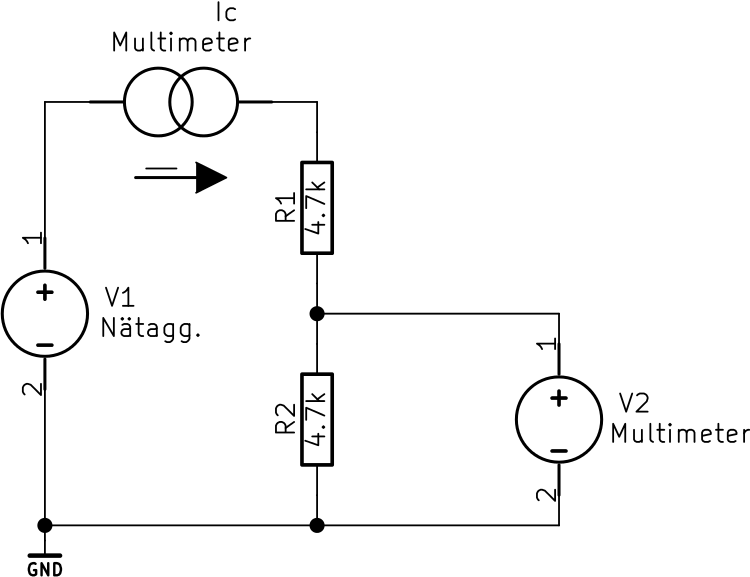
\includegraphics[scale=0.5]{kicad/2-multimeter-schema.png}
    \caption{Spänningsdelarkoppling}
    \label{fig:2-mm-schem}
\end{figure}


\subsection{Mätning av resistans}\label{vdiv}
% ------------------------------------------------------------------------------
\par Mätnoggrannheten för HP34401A är specificerad till $\pm{}0.0035\%$ av
avläst värde + $\pm{}0.0005\%$ av mätområdet. Instrumentet hittar själv det
mätområde bäst lämpat för att uttrycka resultatet med det största möjliga antalet
värdesiffror, som för HP34401A är \si{6\nicefrac{1}{2}} siffror.
\par Mätnoggrannheten för den handhållna Mastech-multimetern kan antas vara
\si{1\%}, vilket är typiskt för multimetrar i den prisklassen.
\par Vi väljer därför att mäta motstånden med bänkmultimetern HP34401A, som ansluts
till motstånden med hjälp av labbsladdar av "banankontakt"-typ och krokodilklämmor.
Vi tänker att kablarnas resistans är negligerbar för det här experimentet.
\\
\par Motståndens resistansvärden väljs godtyckligt inom området \si{1-10\kohm}, 
med \si{10\kohm} för \textbf{R1} och \si{4,7\kohm} för \textbf{R2}.
Motstånden är sannolikt från E24-serien, med en specificerad \si{5\%} tolerans. Vi kan
därför vänta oss att det faktiska värdet kan avvika från det markerade med upp till
$\pm{}5\%$. 
\par Mätresultaten visas i Tabell \ref{restable}.


\begin{table}
    \begin{longtable}[c]{@{}llc@{}}
        \toprule\addlinespace
           & Ideal         & Reell
        \\\addlinespace
        \midrule\endhead
        R1 & \si{10\kohm}  & \si{9,870\kohm}
        \\\addlinespace
        R2 & \si{4,7\kohm} & \si{4,677\kohm}
        \\\addlinespace
        \bottomrule
        \addlinespace
        \caption{Resistansvärden}
        \label{restable}
    \end{longtable}
\end{table}




\subsection{Mätning av spänning och ström}\label{meas_multi}
% ------------------------------------------------------------------------------

\begin{table}
    \begin{longtable}[c]{@{}llc@{}}
        \toprule\addlinespace
                              & Beräknat & Uppmätt
        \\\addlinespace
        \midrule\endhead
        \textbf{I} (\si{\uA}) & 680,27   & 0
        \\\addlinespace
        \textbf{U} (\si{\V})  & 3,1973   & 0
        \\\addlinespace
        \bottomrule
        \addlinespace
        \caption{Spänningsdelaren}
        \label{vdivtable}
    \end{longtable}
\end{table}


% ==============================================================================
% SECTION: RESULTAT
% ==============================================================================
\section{Resultat}\label{setup}
% ==============================================================================
% TODO: Beräkna felvärdet för ideala och reella komponenter:
%       fel(%) = [(uppmätt - förväntat) / förväntat] * 100


\newpage

% ==============================================================================
% SECTION: REFERENSER
% ==============================================================================
\section{Referenser}\label{refs}
% ==============================================================================

\subsection{www}\label{interwebs}
% ------------------------------------------------------------------------------
HP34401A datablad\\
http://literature.cdn.keysight.com/litweb/pdf/5991-1983EN.pdf

\subsection{Trycksaker}\label{literature} %???
% ------------------------------------------------------------------------------
% TODO

%\subsection{Källkod}\label{sourcefiles}
% ------------------------------------------------------------------------------

% ==============================================================================
\end{document}
% ==============================================================================
